%%
%% Author: Berk
%% 3/21/2019
%%

% Preamble
\documentclass[11pt]{article}

% Packages
\usepackage{amsmath}
\usepackage[margin=1in]{geometry}
\usepackage{amsmath,amsthm,amssymb}
\usepackage{comment}
\usepackage[acronyms]{glossaries}
\usepackage{graphicx}
\usepackage{tikz}
\usepackage{tikz-3dplot}
\usetikzlibrary{shapes.geometric}

\newacronym{bsfc}{BSFC}{brake specific fuel consumption}
\newacronym{ceg}{CEG}{Convex Engineering Group}
\newacronym{gp}{GP}{Geometric Program}
\newacronym{mc}{MC}{Monte Carlo}
\newacronym{sp}{SP}{Signomial Program}
\newacronym{rgp}{RGP}{Robust Geometric Program}
\newacronym{rsp}{RSP}{Robust Signomial Program}
\newacronym{ro}{RO}{Robust Optimization}
\newacronym{so}{SO}{Stochastic Optimization}
\newacronym{mdo}{MDO}{Multidisciplinary Design Optimization}
\newacronym{dc}{DC}{difference-of-convex}
\newacronym{nlp}{NLP}{Nonlinear Program}
\newacronym{rhs}{RHS}{right hand side}
\newacronym{lhs}{LHS}{left hand side}
\newacronym{cv}{CV}{coefficient of variation}
\newacronym{srm}{SRM}{solid rocket motor}

\makeglossaries

% Document
\begin{document}

    \title{SDP relaxations for solid rocket motor shape optimization}
    \author{Berk Ozturk}
    \maketitle

    \section{Introduction}
    
    Shape optimization is inherently an infinite-dimensional problem,
for which tractable formulations are of particular interest.
    It appears in a range of problems in aerospace design, and most notably
    aerostructural optimization which has been the bread-and-butter of the \gls{mdo} field.

	These is very little literature, if any, on solid rocket conceptual design,
for several reasons. (1) The physics governing internal reactive flow is extremely complex,
and there are no open-source tools that don't require domain knowledge and
can efficiently simulate such a scenario.
(2) There are few entities that design and build solid rocket motors, and since they have
large amounts of resources and time and little competition there has been no impetus
improve solid rocket design methods. (3) Solid rocket motors are relatively limited
in capability because their burn rate is almost completely uncontrollable other
than by properly designing the internal geometry of the rocket or actuating the
throat of the nozzle. For this reason liquid propellant rockets have been preferred for
many applications. (4) Rocket design is often proprietary due to arms regulations.

    \section{Approach}
    
    I am developing a two-stage approach to the \gls{srm} design problem. The first stage is a 1D quasi-steady rocket optimization model, which determines both the internal flow quantities and a basic description of the internal geometry. I have already developed this model 
    
\tdplotsetmaincoords{50}{130}
\tdplotsetrotatedcoords{0}{90}{0}

\begin{figure}
\begin{center}
\begin{tikzpicture}[tdplot_main_coords]
    \draw[thick,->] (0,0,0) -- (1,0,0) node[anchor=north east]{$l$};
    \draw[thick,->] (0,0,0) -- (0,-1,0) node[anchor=south west]{$r$};
    \draw[thick,dashed] (0,0,0) -- (-4,0,0) node[anchor=north west]{$$};
    % Blue circles
    \tdplotdrawarc[tdplot_rotated_coords, color=blue]{(0,0,-4)}{2}{0}{360}{anchor=south west}{$\pi r^2$};
    \tdplotdrawarc[tdplot_rotated_coords, color=blue]{(0,0,0)}{2}{0}{360}{anchor=south west}{$$};
    % Blue dashed lines
    \draw[thick,dashed,color=blue] (0,-1.414,1.414) -- (-4,-1.414,1.414) node[anchor=south east]{$l_{\rm{sec}}$};
    \draw[thick,dashed,color=blue] (0,1.414,-1.414) -- (-4,1.414,-1.414) node[anchor=north west]{$l_{\rm{sec}}$};

    % Tophalf, top circle
    \tdplotdrawarc[tdplot_rotated_coords, color=red]{(-0.25,0.25,-4)}{1}{25}{248}{anchor=north west}{$$};
    % Top half, bottom circle
    \tdplotdrawarc[tdplot_rotated_coords, color=red]{(0.25,-0.25,-4)}{1}{205}{428}{anchor=north west, right=0.5cm, above=0.5cm}{$A_{in}$};
    % Bottom half, top circle
    \tdplotdrawarc[tdplot_rotated_coords, color=red]{(-0.25,0.25,0)}{1.25}{28}{243}{anchor=north west}{$$};
    % Bottom half, bottom circle
    \tdplotdrawarc[tdplot_rotated_coords, color=red]{(0.25,-0.25,0)}{1.25}{208}{425}{anchor=north west, right=0.5cm}{$A_{out}$};

    % Red dashed lines
    \draw[thick,dashed,color=red] (0,-0.85,0.85) -- (-4,-0.67,0.67) node[anchor=south east]{$$};
    \draw[thick,dashed,color=red] (0,0.85,-0.85) -- (-4,0.67,-0.67) node[anchor=north west]{$$};
\end{tikzpicture}
\end{center}
    \caption{Labeling of a single section of the rocket. }
    \label{fig:SRMsection}
\end{figure}

This first-stage optimization problem takes in the following inputs:
    \begin{itemize}
    \item Coarse time and spatial discretization of the rocket sections
    \item The desired thrust profile of the rocket
    \item Bounds on the rocket external dimensions, if desired
    \item Material properties of the propellant  
    \end{itemize}
    
Figure~\ref{fig:SRMsection} shows a potential cross-section of a \gls{srm}.
The rocket is partitioned into $n_x$ of these sections that evolve in $n_t$ timesteps. The physical model assumes quasi-steady flow during each timestep, where the fluid travels strictly
in the $l$ direction, and the conservation laws are enforced at
each bore cross-sectional area $A$.

The output variables of this model are:
    
    \begin{itemize}
    \item The material properties of the fuel burned in a given section in one timestep
        \begin{itemize}
        \item Porosity of fuel
        \item Mass fraction of propellant
        \item Mass fraction of accelerant
        \item Mass fraction of filler
        \end{itemize}
    \item The circumferences of shapes of $A_{in}$ and $A_{out}$
    \item The cross-sectional areas of $A_{in}$ and $A_{out}$
    \end{itemize}
    
The idea is to take these output variables, and map them onto a series of 
non-intersecting univariate polynomials $p(\theta, t)$ which describe the internal geometry of the rocket. 

To give context about the kinds of shapes that could result, see Figure~\ref{fig:potentialShapes}. The sky is really the limit. The hope is that this problem has an SDP relaxation that can find polynomials that can fulfill the constraints, at a minimum in a least-squares sense, since feasibility is not guaranteed. 

\begin{figure}
\centering
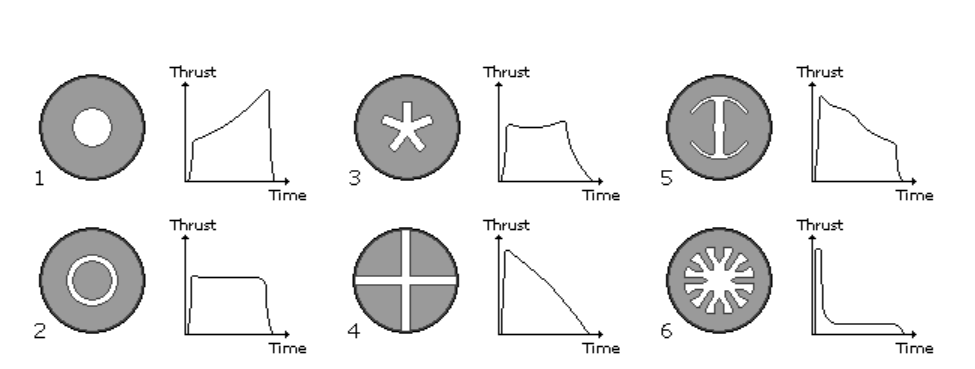
\includegraphics[width=0.7\linewidth]{figures/potentialShapes.png}
\label{fig:potentialShapes}
\caption{Different thrust profiles may result in very different potential internal configurations of the rocket. Image courtesy of Robert A. Braeunig.}

\end{figure}

\section{Basis functions}

Since I will be optimizing the shapes over the units circle and scaling the result to fit into the rocket shell in question, I will be using a peri

\section{Constraints}

The constraints are imposed at $n_x+1$ cross-sections. The surface geometry in between the sections will be described through interpolation. 

\begin{itemize}
\item \textbf{The integral difference between the cross-sectional areas of the shape must be equal to the fuel burnt in a given time step. }
\item \textbf{The shapes must never intersect.} Since the flame front must strictly regress as a result of burning, the polynomials describing the shapes must have no common roots. Knowing that the 
\item\textbf{The shapes must never intersect the unit circle.} Since fuel can only be contained inside the casing of the rocket, we set an upper bound on the polynomials. 
\item \textbf{Regularity conditions on the shape of the polynomials.} Not sure what form these will take, but the shapes of the polynomials must `follow' each other. 
\end{itemize}




\end{document}
